\documentclass{standalone}
\usepackage{tikz, ifthen}
\usepackage{amsmath}

\begin{document}

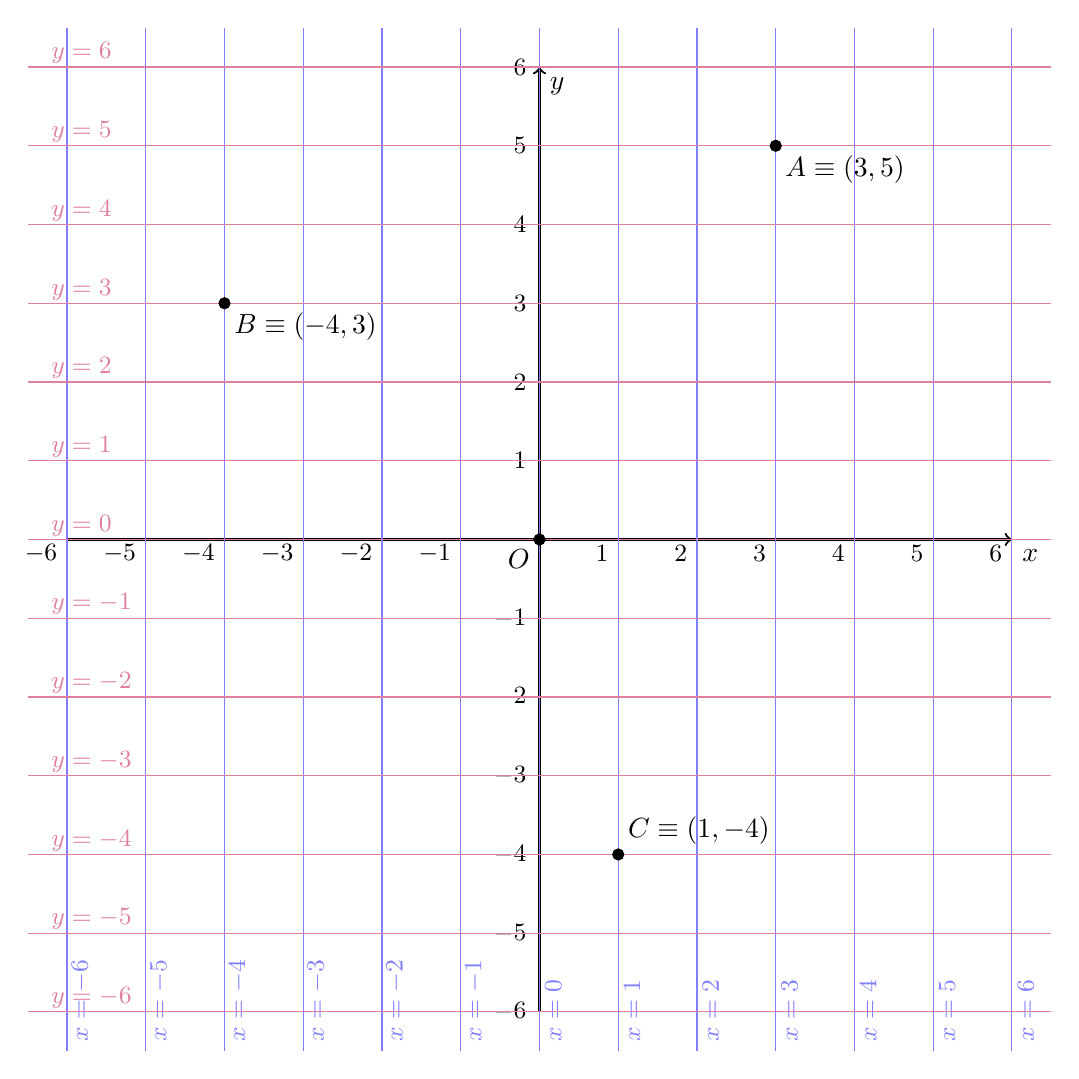
\begin{tikzpicture}
    
    % Center of the circle
    \def\xmin{-6}
    \def\xmax{6}
    \def\ymin{-6}
    \def\ymax{6}
    \def\dx{.5}
    \def\dy{.5}
    \def\xminb{\xmin-\dx}
    \def\xmaxb{\xmax+\dx}
    \def\yminb{\ymin-\dy}
    \def\ymaxb{\ymax+\dy}
    \def\xo{2}     % translation, x
    \def\yo{1.5}   % translation, y
    \def\xpmin{-6}
    \def\xpmax{ 6}
    \def\ypmin{-5.5}
    \def\ypmax{ 5.5}

    % Fill outside region
    \clip (\xminb, \yminb) rectangle (\xmaxb, \ymaxb);
%   \begin{scope}
%       \clip (\xminb, \yminb) rectangle (\xmaxb, \ymaxb);
%       % \fill[gray!30] (\xmin, \ymin) rectangle (5, \ymax);
%       % \fill[gray!30] (center) circle (3);
%   \end{scope}

%   % Draw grid
%   \draw[step=1., gray!60, ultra thin] (\ymin, \xmin) grid (\ymax, \ymax); % Visible grid with lighter color
    
    % Axes, x
    \draw[->, thick, black] (\xmin, 0) -- (\xmax, 0) node[below right] {$x$};
    \draw[->, thick, black] (0, \ymin) -- (0, \ymax) node[below right] {$y$};
    % Axis ticks
    \foreach \x in {\xmin,..., \xmax}{
        \ifthenelse{ \x = 0 }{}{\draw[black] (\x, -0.1) -- (\x, +0.1) node[below=8pt, left=0pt] {\small $\x$};}
    }
    \foreach \y in {\ymin,..., \ymax}{
        \ifthenelse{ \y = 0 }{}{\draw[black] (-0.1, \y) -- (0.1, \y) node[left=4pt] {\small $\y$};}
    }
    
    % Axis ticks
    \foreach \x in {\xmin,..., \xmax}{
        \draw[blue!50, thin] (\x, \yminb)  node[right=5pt, rotate=90] {\small $x=\x$} -- (\x, \ymaxb);
    }
    \foreach \y in {\ymin,..., \ymax}{
        \draw[purple!50, thin] (\xminb,\y)  node[above=5pt, right=5pt, rotate=0] {\small $y=\y$} -- (\xmaxb,\y);
    }

    % Origin
    \filldraw[black] (0,0) circle (2pt) node[below left] {$O$};

%   \filldraw[blue]  (3,5) circle (1pt) node[below right] {$\equiv (3,5)$};
    \filldraw[black] (3,5) circle (2pt) node[below right] {$A \equiv (3,5)$};

%   \filldraw[blue]  (-4,3) circle (1pt) node[below right] {$\equiv (-4,3)$};
    \filldraw[black] (-4,3) circle (2pt) node[below right] {$B \equiv (-4,3)$};

%   \filldraw[blue]   (1,-4) circle (0pt) node[above right=8pt] {$\qquad \ 1$};
%   \filldraw[purple] (1,-4) circle (0pt) node[above right=8pt] {$\qquad \quad \ -4$};
    \filldraw[black]  (1,-4) circle (2pt) node[above right] {$C \equiv (1,-4)$};

%   % Foci
%   \filldraw[blue] (\xa, \ya) circle (2pt) node[above right] {$0$};
%   \filldraw[blue] (\xb, \yb) circle (2pt) node[above right] {$2$};
    
\end{tikzpicture}

\end{document}
